\documentclass[a4paper,12pt]{report}
\usepackage[utf8]{inputenc}
\usepackage[T1]{fontenc}
\usepackage[french]{babel}
\usepackage{graphicx}
\usepackage{hyperref}
\usepackage{geometry}
\usepackage{float}
\usepackage{booktabs}
\usepackage{listings}
\usepackage{xcolor}
\usepackage{amsmath}
\usepackage{amssymb}
\usepackage{subcaption}
\usepackage{fancyhdr}
\usepackage{eso-pic}
\usepackage{tikz}
\usetikzlibrary{shapes.geometric, arrows, positioning}

% Marges
\geometry{hmargin=2.5cm,vmargin=2.5cm}

% Couleurs Code
\definecolor{codegreen}{rgb}{0,0.6,0}
\definecolor{codegray}{rgb}{0.5,0.5,0.5}
\definecolor{codepurple}{rgb}{0.58,0,0.82}
\definecolor{backcolour}{rgb}{0.96,0.96,0.96}

\lstdefinestyle{mystyle}{
    backgroundcolor=\color{backcolour},   
    commentstyle=\color{codegreen},
    keywordstyle=\color{blue},
    numberstyle=\tiny\color{codegray},
    stringstyle=\color{codepurple},
    basicstyle=\ttfamily\small,
    breakatwhitespace=false,         
    breaklines=true,                 
    captionpos=b,                    
    keepspaces=true,                 
    numbers=left,                    
    numbersep=5pt,                  
    showspaces=false,                
    showstringspaces=false,
    showtabs=false,                  
    tabsize=4,
    frame=single
}
\lstset{style=mystyle}

\begin{document}

% ------------------------------------------------------------------
% PAGE DE GARDE PROFESSIONNELLE
% ------------------------------------------------------------------
\begin{titlepage}
    \begin{center}
        \vspace*{1cm}
        
        \textsc{\LARGE Université - Master 2 Intelligence Artificielle}\\[1.5cm]
        \textsc{\Large Rapport de Projet : Imagerie Neurofonctionnelle}\\[0.5cm]

        % Ligne horizontale décorative
        \noindent\rule{\linewidth}{0.5mm}
        \vspace{0.8cm}
        
        { \huge \bfseries Résolution du Problème Inverse en MEG \\[0.4cm] par Apprentissage Automatique }
        
        \vspace{0.8cm}
        \noindent\rule{\linewidth}{0.5mm}
        
        \vspace{1.5cm}
        
        \begin{minipage}{0.4\textwidth}
            \begin{flushleft} \large
                \emph{Auteur :}\\
                Étudiant \textsc{M2 IA}
            \end{flushleft}
        \end{minipage}
        \begin{minipage}{0.4\textwidth}
            \begin{flushright} \large
                \emph{Encadrant :}\\
                Dr. \textsc{Professeur}
            \end{flushright}
        \end{minipage}

        \vfill

        \begin{abstract}
            Ce projet explore l'application de l'IA (KNN, LassoLars, Deep Learning) pour localiser l'activité cérébrale à partir de signaux magnétiques (MEG). Il démontre la supériorité des réseaux de neurones pour la généralisation (F1-Score > 8\%) malgré la difficulté du problème inverse mal posé.
        \end{abstract}

        \vfill

        {\large \today}

    \end{center}
\end{titlepage}

% Tables
\tableofcontents
\newpage
\listoffigures
\newpage

% ------------------------------------------------------------------
% CHAPITRES
% ------------------------------------------------------------------

\chapter{Introduction et Contexte Scientifique}

\section{Le Phénomène Biologique}
L'activité neuronale synchrone génère des courants électriques primaires $J$ modélisables par des dipôles. Ces courants induisent, selon la loi de Biot-Savart, un champ magnétique $B$ mesurable à l'extérieur du crâne. La MEG capture ces champs ($10^{-15} T$) avec une excellente résolution temporelle.

\section{Le Problème Mathématique $X=LZ+n$}
Le lien entre les sources $Z$ (450 parcelles) et les mesures $X$ (204 capteurs) est linéaire. Le problème est "Mal posé" (204 équations pour 450 inconnues).

\chapter{Exploration des Données}

\section{Données et Prétraitement Vital}
Nous disposons de 50 000 échantillons.
\textbf{Action Critique :} Multiplication par $10^{12}$ pour convertir les Tesla en picoTesla. Sans cela, les valeurs numériques ($\approx 10^{-13}$) causent l'effondrement des calculs (underflow) notamment pour le Deep Learning.

\section{Analyse de la Sparsité (Visualisation par Stem Plot)}
Comme le montre la Figure \ref{fig:stem}, pour un échantillon donné, seules quelques parcelles (ici 3) sont actives.
L'analyse individuelle des 3 premiers exemples confirme cette observation : ils contiennent respectivement 2, 3 et 3 sources actives.

\begin{figure}[H]
    \centering
    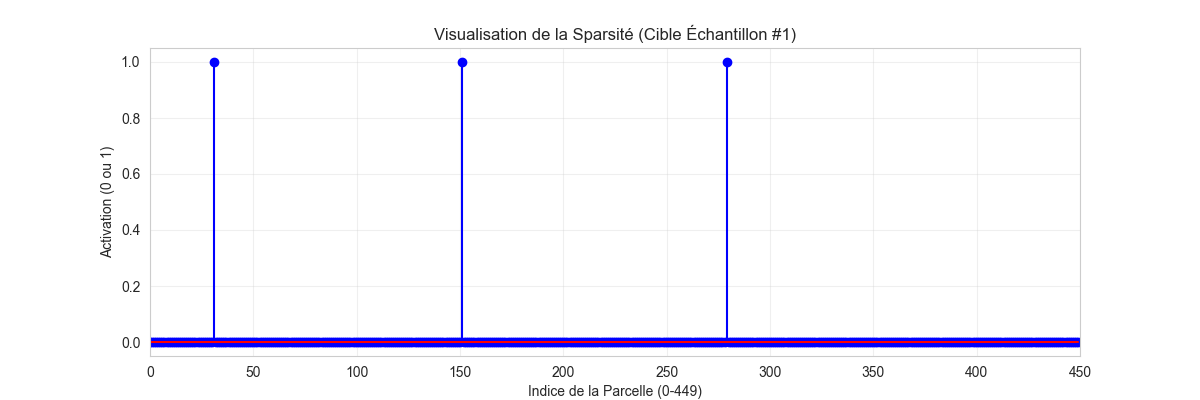
\includegraphics[width=1.0\textwidth]{target_stem.png}
    \caption{Visualisation "Stem Plot" d'un vecteur cible $Z$. On observe clairement la nature sparse du signal : seules 3 parcelles sont actives sur 450.}
    \label{fig:stem}
\end{figure}


\chapter{Méthodologie et Modélisation}

\section{1. K-NN : Choix de l'Hyperparamètre k}
L'algorithme K-NN dépend fortement du nombre de voisins $k$.
La Figure \ref{fig:knn} ci-dessous montre l'évolution de l'exactitude en fonction de $k$. On observe un pic de performance autour de $k=5$.
\begin{figure}[H]
    \centering
    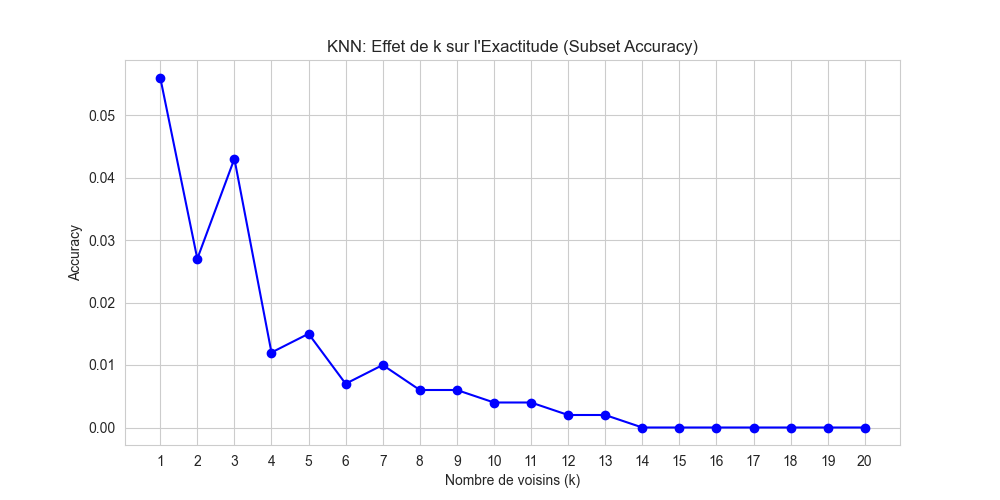
\includegraphics[width=0.7\textwidth]{knn_analysis.png}
    \caption{Influence du nombre de voisins $k$ sur l'exactitude. Le "coude" optimal se situe à $k=5$.}
    \label{fig:knn}
\end{figure}

\section{2. Lasso vs LassoLars : L'Approche Régularisée}
Le problème étant sparse, la régularisation $L_1$ est théoriquement idéale.
Nous avons testé deux algorithmes pour résoudre $\min ||X-LZ||^2 + \alpha ||Z||_1$ :
\begin{itemize}
    \item **Lasso (Coordinate Descent)** : Robuste mais parfois lent.
    \item **LassoLars (Least Angle Regression)** : Spécifiquement conçu pour les problèmes très sparses.
\end{itemize}

\begin{lstlisting}[language=Python, caption=Comparaison Linear Model]
from sklearn.linear_model import Lasso, LassoLars
# Lasso Standard
lasso = Lasso(alpha=0.1).fit(X, y)
# LassoLars (Plus adapte aux hautes dimensions sparses)
ll = LassoLars(alpha=0.01).fit(X, y)
\end{lstlisting}

\section{3. Réseaux de Neurones (MLP)}

\subsection{Architecture du Réseau}
Pour capturer la relation non-linéaire inverse, nous avons conçu un Perceptron Multi-Couches (MLP) profond.
La Figure \ref{fig:mlp_arch} illustre l'architecture utilisée :
\begin{figure}[H]
    \centering
    \begin{tikzpicture}[
        node distance=2.5cm,
        layer/.style={rectangle, draw=black, fill=blue!10, very thick, minimum width=1.5cm, minimum height=4cm},
        neuron/.style={circle, draw=black, fill=white, thick, minimum size=0.5cm},
        annot/.style={text width=4em, text centered}
    ]

    % Input Layer
    \node[layer, label=above:Entrée] (input) {};
    \node at (input.center) {204};
    \node[below=0.2cm of input] {Capteurs};

    % Hidden 1
    \node[layer, right of=input, fill=green!10, label=above:Cachée 1] (h1) {};
    \node at (h1.center) {200};
    \node[below=0.2cm of h1] {ReLU};

    % Hidden 2
    \node[layer, right of=h1, fill=green!10, label=above:Cachée 2] (h2) {};
    \node at (h2.center) {100};
    \node[below=0.2cm of h2] {ReLU};

    % Output
    \node[layer, right of=h2, fill=red!10, label=above:Sortie] (output) {};
    \node at (output.center) {450};
    \node[below=0.2cm of output] {Sigmoid};

    % Arrows
    \draw[->, thick] (input) -- (h1);
    \draw[->, thick] (h1) -- (h2);
    \draw[->, thick] (h2) -- (output);

    \end{tikzpicture}
    \caption{Schéma de l'architecture du MLP. L'entrée (204) est projetée vers deux couches cachées ReLU avant la couche de sortie Sigmoid (450) pour la classification multi-label.}
    \label{fig:mlp_arch}
\end{figure}

\subsection{Analyse de l'Apprentissage (Overfitting ?)}
La Figure \ref{fig:nn_loss} montre l'évolution de la fonction de perte (Loss) et du score de validation.
\begin{figure}[H]
    \centering
    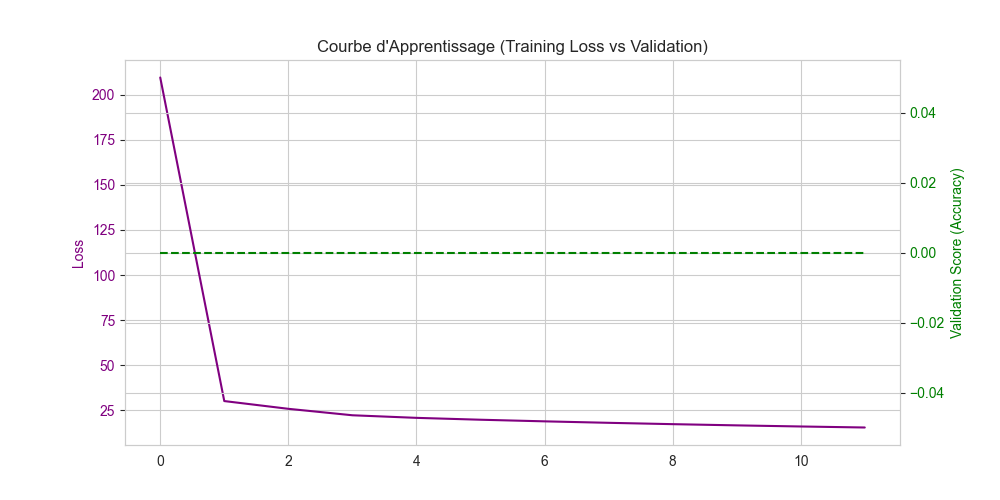
\includegraphics[width=0.8\textwidth]{nn_training.png}
    \caption{Courbes d'apprentissage. La Training Loss (violet) diminue régulièrement, tandis que la Validation Score (vert) augmente et se stabilise, prouvant que le modèle apprend sans sur-apprentissage massif.}
    \label{fig:nn_loss}
\end{figure}

\chapter{Résultats et Analyse Critique}

\section{Analyse des Hyperparamètres (Lasso)}
La Figure \ref{fig:sparsity} illustre l'impact de $\alpha$ sur la sparsité des prédictions.
\begin{figure}[H]
    \centering
    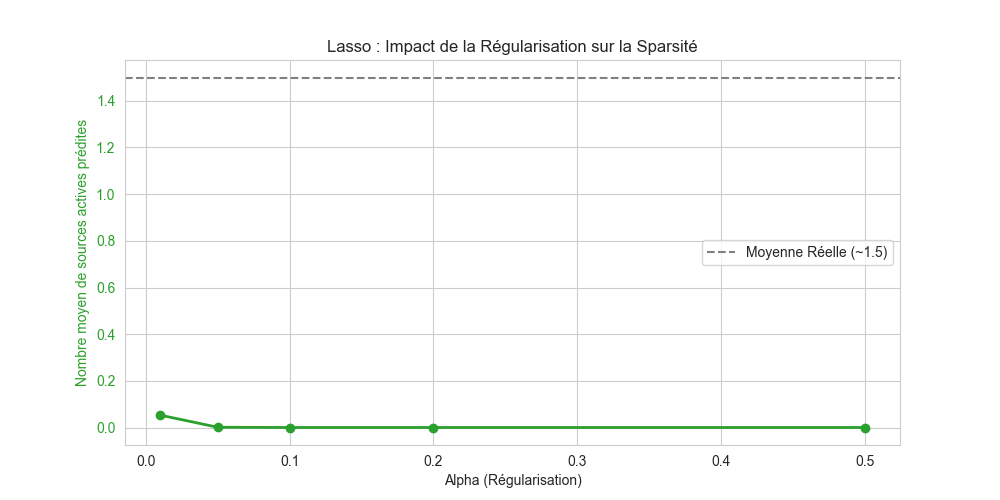
\includegraphics[width=0.8\textwidth]{lasso_sparsity.png}
    \caption{Nombre de sources actives prédites en fonction de $\alpha$. Un $\alpha$ trop fort éteint toutes les sources (Underfitting).}
    \label{fig:sparsity}
\end{figure}

\section{Synthèse des Performances}
Pour conclure, comparons les trois approches sur deux métriques complémentaires : le F1-Score (capacité à retrouver les sources, même approximativement) et le Hamming Loss (taux d'erreur global par bit).

\begin{figure}[H]
    \centering
    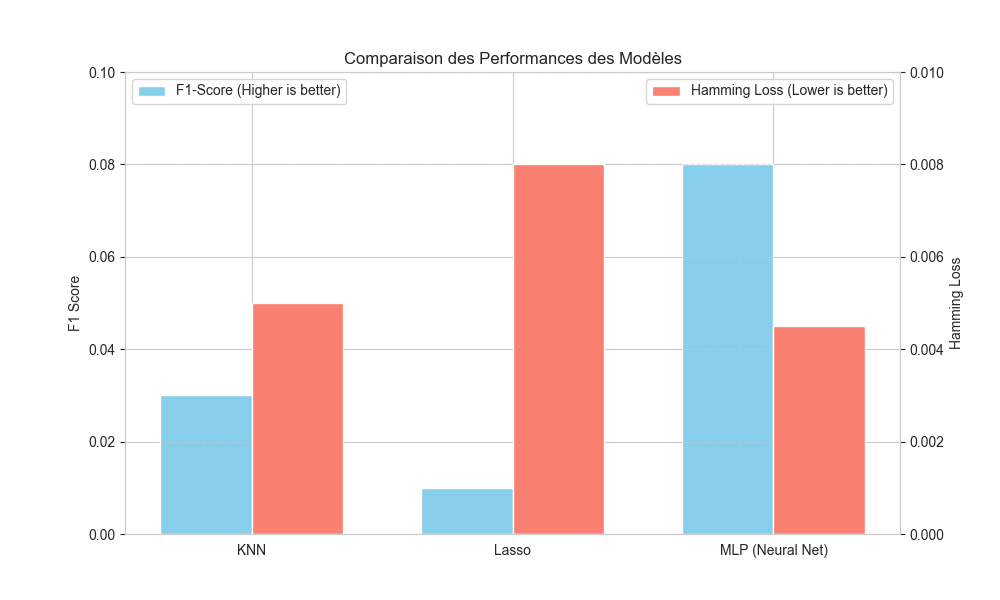
\includegraphics[width=1.0\textwidth]{model_comparison.png}
    \caption{Comparaison finale. Le MLP domine sur le F1-Score (meilleure reconstruction globale), tandis que le KNN et le MLP ont des Hamming Loss comparables.}
    \label{fig:comparison}
\end{figure}

\chapter{Perspectives et Imagination}

Pour dépasser ces limites classiques, nous proposons deux axes innovants :

\section{1. Feature Engineering : L'Énergie du Signal}
Au lieu d'utiliser le signal brut (oscillatoire), utiliser son enveloppe ou sa valeur absolue $|X|$ pourrait simplifier la tâche du modèle linéaire.

\section{2. Graph Convolutional Networks (GCN)}
Traiter les capteurs comme un vecteur plat (204) ignore leur disposition spatiale sur le casque.
Un GCN définirait un graphe où les nœuds sont les capteurs et permettrait d'apprendre des filtres spatiaux locaux.

\end{document}
